\documentclass[tikz, border=15pt]{standalone}
\usepackage[utf8]{inputenc}
\usepackage{amsmath}

\begin{document}

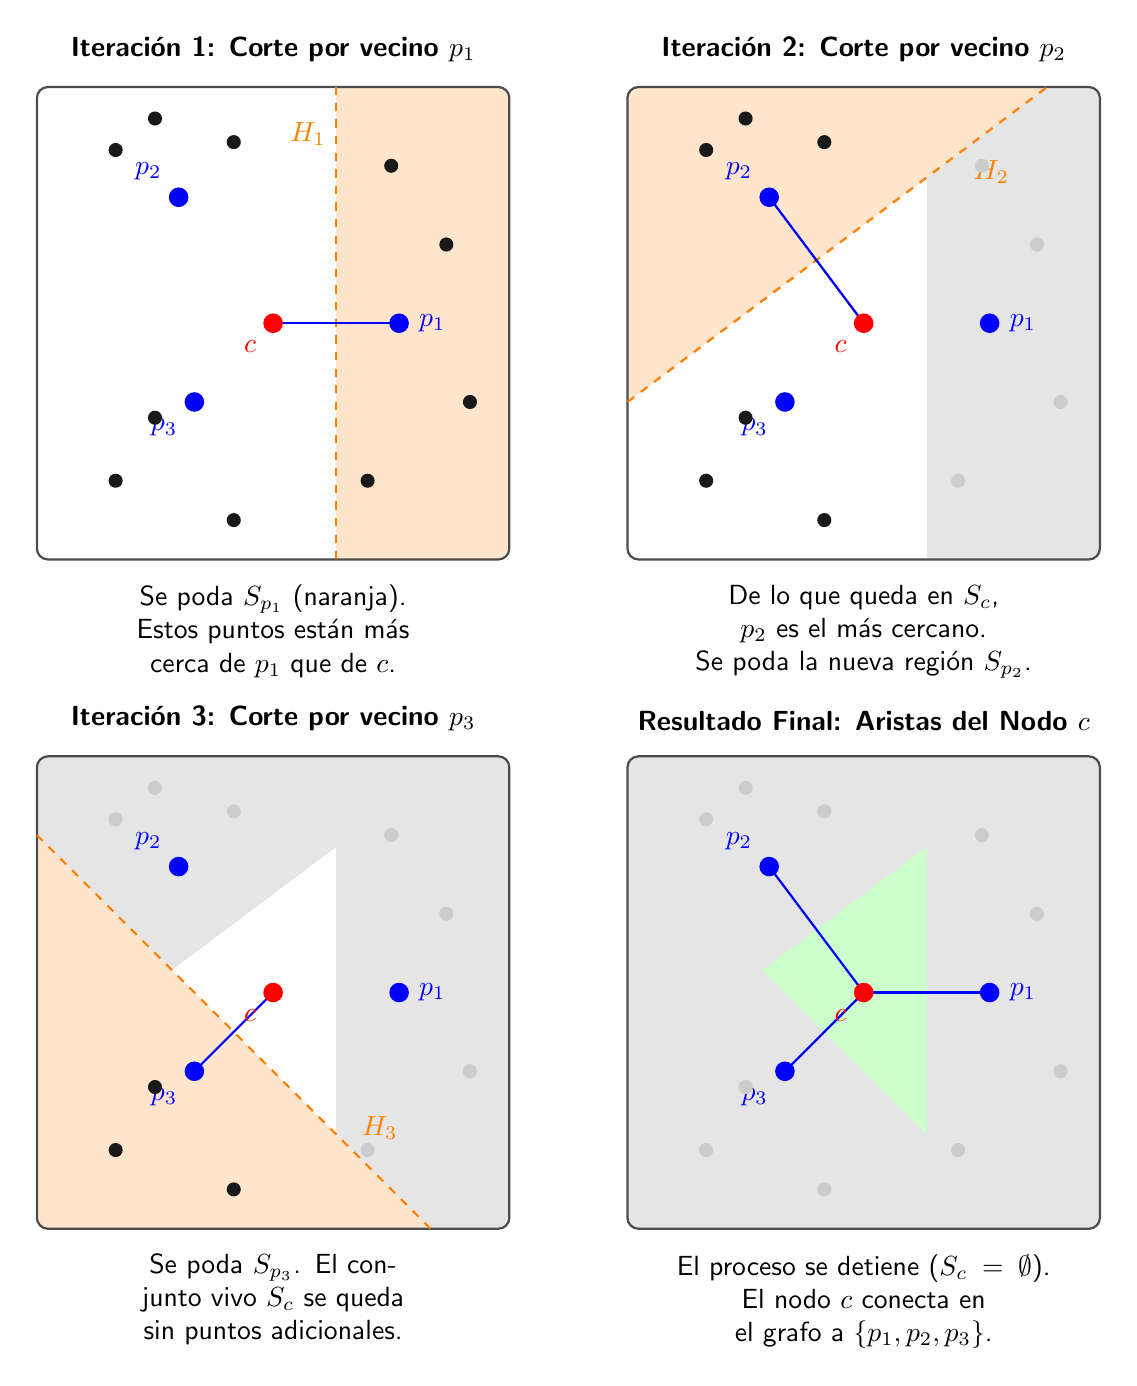
\begin{tikzpicture}[
    font=\sffamily,
    % Estilos de los nodos
    cnode/.style={circle, fill=red, inner sep=2.5pt},
    pnode/.style={circle, fill=blue, inner sep=2.5pt},
    activep/.style={circle, fill=black!90, inner sep=1.8pt},
    prunedp/.style={circle, fill=black!20, inner sep=1.8pt},
    % Estilos de líneas y marcos
    bisect/.style={thick, dashed, orange},
    conn/.style={thick, blue},
    box/.style={thick, draw=black!70, rounded corners=4pt}
]

% ==========================================
% MACROS PARA MANTENER LA CONSISTENCIA
% ==========================================
% Nodos principales (Centro y vecinos elegidos)
\newcommand{\drawpnodes}{
    \node[pnode, label={[blue]right:$p_1$}] (p1) at (1.6, 0) {};
    \node[pnode, label={[blue]above left:$p_2$}] (p2) at (-1.2, 1.6) {};
    \node[pnode, label={[blue]below left:$p_3$}] (p3) at (-1, -1) {};
}
\newcommand{\drawcnode}{
    \node[cnode, label={[red]below left:$c$}] (c) at (0,0) {};
}

% Puntos que pertenecen a Sp1 (Podados en Iteración 1)
\newcommand{\drawpOnepoints}[1]{
    \node[#1] at (1.5, 2) {};
    \node[#1] at (2.2, 1) {};
    \node[#1] at (2.5, -1) {};
    \node[#1] at (1.2, -2) {};
}
% Puntos que pertenecen a Sp2 (Podados en Iteración 2)
\newcommand{\drawpTwopoints}[1]{
    \node[#1] at (-2, 2.2) {};
    \node[#1] at (-1.5, 2.6) {};
    \node[#1] at (-0.5, 2.3) {};
}
% Puntos que pertenecen a Sp3 (Podados en Iteración 3)
\newcommand{\drawpThreepoints}[1]{
    \node[#1] at (-2, -2) {};
    \node[#1] at (-1.5, -1.2) {};
    \node[#1] at (-0.5, -2.5) {};
}

% ==========================================
% PANEL 1: ITERACIÓN 1
% ==========================================
\begin{scope}[shift={(0,0)}]
    % Recortar para que el sombreado no salga del cuadro
    \begin{scope}
        \clip[rounded corners=4pt] (-3,-3) rectangle (3,3);
        % Región Sp1 (x > 0.8)
        \fill[orange!20] (0.8, -4) rectangle (4, 4);
    \end{scope}
    
    \draw[box] (-3,-3) rectangle (3,3);
    
    % Hiperplano H1 (x = 0.8)
    \draw[bisect] (0.8, -3) -- (0.8, 3) node[pos=0.9, left, orange] {$H_1$};
    \draw[conn] (0,0) -- (1.6,0);
    
    \drawpnodes \drawcnode
    \drawpOnepoints{activep} \drawpTwopoints{activep} \drawpThreepoints{activep}
    
    \node[anchor=south] at (0, 3.2) {\textbf{Iteración 1: Corte por vecino $p_1$}};
    \node[anchor=north, align=center, text width=6cm] at (0, -3.2) {Se poda $S_{p_1}$ (naranja).\\Estos puntos están más cerca de $p_1$ que de $c$.};
\end{scope}

% ==========================================
% PANEL 2: ITERACIÓN 2
% ==========================================
\begin{scope}[shift={(7.5,0)}]
    \begin{scope}
        \clip[rounded corners=4pt] (-3,-3) rectangle (3,3);
        % Sp1 ya fue podado (gris)
        \fill[black!10] (0.8, -4) rectangle (4, 4);
        % Región Sp2 (y > 0.75x + 1.25)
        \fill[orange!20] (-4, -1.75) -- (4, 4.25) -- (-4, 4.25) -- cycle;
    \end{scope}
    
    \draw[box] (-3,-3) rectangle (3,3);
    
    % Hiperplano H2 (y = 0.75x + 1.25)
    \draw[bisect] (-3, -1) -- (2.33, 3) node[pos=0.8, below right, orange] {$H_2$};
    \draw[conn] (0,0) -- (-1.2, 1.6);
    
    \drawpnodes \drawcnode
    \drawpOnepoints{prunedp} \drawpTwopoints{activep} \drawpThreepoints{activep}
    
    \node[anchor=south] at (0, 3.2) {\textbf{Iteración 2: Corte por vecino $p_2$}};
    \node[anchor=north, align=center, text width=6cm] at (0, -3.2) {De lo que queda en $S_c$, $p_2$ es el más cercano.\\Se poda la nueva región $S_{p_2}$.};
\end{scope}

% ==========================================
% PANEL 3: ITERACIÓN 3
% ==========================================
\begin{scope}[shift={(0,-8.5)}]
    \begin{scope}
        \clip[rounded corners=4pt] (-3,-3) rectangle (3,3);
        % Zonas previas en gris
        \fill[black!10] (0.8, -4) rectangle (4, 4);
        \fill[black!10] (-4, -1.75) -- (4, 4.25) -- (-4, 4.25) -- cycle;
        % Región Sp3 (y < -x - 1)
        \fill[orange!20] (-4, 3) -- (4, -5) -- (-4, -5) -- cycle;
    \end{scope}
    
    \draw[box] (-3,-3) rectangle (3,3);
    
    % Hiperplano H3 (y = -x - 1)
    \draw[bisect] (-3, 2) -- (2, -3) node[pos=0.8, above right, orange] {$H_3$};
    \draw[conn] (0,0) -- (-1, -1);
    
    \drawpnodes \drawcnode
    \drawpOnepoints{prunedp} \drawpTwopoints{prunedp} \drawpThreepoints{activep}
    
    \node[anchor=south] at (0, 3.2) {\textbf{Iteración 3: Corte por vecino $p_3$}};
    \node[anchor=north, align=center, text width=6cm] at (0, -3.2) {Se poda $S_{p_3}$. El conjunto vivo $S_c$ se queda \\ sin puntos adicionales.};
\end{scope}

% ==========================================
% PANEL 4: RESULTADO FINAL (GRAFO HSP)
% ==========================================
\begin{scope}[shift={(7.5,-8.5)}]
    \begin{scope}
        \clip[rounded corners=4pt] (-3,-3) rectangle (3,3);
        % Todo el espacio exterior es gris
        \fill[black!10] (-4, -4) rectangle (4, 4);
        % La celda que sobrevive S_c (intersección exacta de los semiespacios)
        \fill[green!20] (0.8, 1.85) -- (-1.285, 0.285) -- (0.8, -1.8) -- cycle;
    \end{scope}
    
    \draw[box] (-3,-3) rectangle (3,3);
    
    % Aristas finales del grafo
    \draw[conn, thick] (0,0) -- (1.6, 0);
    \draw[conn, thick] (0,0) -- (-1.2, 1.6);
    \draw[conn, thick] (0,0) -- (-1, -1);
    
    \drawpnodes \drawcnode
    \drawpOnepoints{prunedp} \drawpTwopoints{prunedp} \drawpThreepoints{prunedp}
    
    \node[anchor=south] at (0, 3.2) {\textbf{Resultado Final: Aristas del Nodo $c$}};
    \node[anchor=north, align=center, text width=6cm] at (0, -3.2) {El proceso se detiene ($S_c = \emptyset$).\\El nodo $c$ conecta en el grafo a $\{p_1, p_2, p_3\}$.};
\end{scope}

\end{tikzpicture}

\end{document}
